%%%
% Plantilla de Memoria
%%%

%----------------------------------------------------------------------------------------
%	PAQUETES Y CONFIGURACIÓN DEL DOCUMENTO
%----------------------------------------------------------------------------------------

%%% Configuración del papel.
% microtype: Tipografía.
% mathpazo: Usa la fuente Palatino.
\documentclass[a4paper,11pt]{article}	
\usepackage[protrusion=true,expansion=true]{microtype}
\usepackage{mathpazo}

% Indentación de párrafos para Palatino
\setlength{\parindent}{0pt}
  \parskip=8pt
\linespread{1.02} % Change line spacing here, Palatino benefits from a slight increase by default


%%% Castellano.
% noquoting: Permite uso de comillas no españolas.
% lcroman: Permite la enumeración con numerales romanos en minúscula.
% fontenc: Usa la fuente completa para que pueda copiarse correctamente del pdf.
\usepackage[spanish,es-noquoting,es-lcroman]{babel}
\usepackage[utf8]{inputenc}
\usepackage[T1]{fontenc}
\usepackage{listings}
\usepackage{booktabs}
\usepackage{fancyvrb}
\usepackage{hyperref}
\usepackage{graphicx}
\selectlanguage{spanish}
\graphicspath{ {./img/} }
\hypersetup{
     colorlinks=true,
     linkcolor=blue,
     filecolor=blue,
     citecolor = black,      
     urlcolor=cyan,
     }

%%% Gráficos
\usepackage{graphicx} % Required for including pictures
\usepackage{wrapfig} % Allows in-line images
\usepackage[usenames,dvipsnames]{color} % Coloring code
\usepackage{float} % Force float position

%%% Matemáticas
\usepackage{amsmath}
\usepackage{amssymb}

%%% Bibliografía
\makeatletter
\renewcommand\@biblabel[1]{\textbf{#1.}} % Change the square brackets for each bibliography item from '[1]' to '1.'
\renewcommand{\@listI}{\itemsep=0pt} % Reduce the space between items in the itemize and enumerate environments and the bibliography

\definecolor{dkgreen}{rgb}{0,0.6,0}
\definecolor{gray}{rgb}{0.5,0.5,0.5}
\definecolor{mauve}{rgb}{0.58,0,0.82}

\lstset{frame=tb,
  language=Matlab,
  aboveskip=1mm,
  belowskip=1mm,
  showstringspaces=false,
  columns=flexible,
  basicstyle={\small\ttfamily},
  numbers=none,
  numberstyle=\tiny\color{gray},
  keywordstyle=\color{blue},
  commentstyle=\color{dkgreen},
  stringstyle=\color{mauve},
  breaklines=true,
  breakatwhitespace=true,
  tabsize=2
}

\renewcommand{\lstlistingname}{Listado}% Listing -> Algorithm
\renewcommand\spanishtablename{Tabla}
\renewcommand{\arraystretch}{1.2}

%----------------------------------------------------------------------------------------
%	TÍTULO
%----------------------------------------------------------------------------------------
% Configuraciones para el título.
% El título no debe editarse aquí.
\renewcommand{\maketitle}{
  \begin{center} % Right align
  
  {\huge\@title} % Increase the font size of the title
  \vspace{180pt} % Some vertical space between the title and author name
  
  {\Large\@author} % Author name
  \\\@date % Date
  \newpage
  \end{center}
}

%% Título
\title{\textbf{Fundamentos Matemáticos y Físicos para Informática Gráfica} % Title
\bigbreak
Memoria de Laboratorio del\\Módulo 2: Matemáticas} % Subtitle
\author{\textbf{Félix de las Pozas Álvarez} % Author
{- felix.delaspozas@urjc.es}\\
\textbf{Gael Rial Costas} % Author
{- gael.rial.costas@urjc.es}\\
\textbf{Antonio Arian Silaghi} % Author
{- aa.silaghi.2018@alumnos.urjc.es}\\
\vspace{2cm}
\bigbreak
\textit{Máster Universitario en Informática Gráfica, \\Juegos y Realidad Virtual 2022/2023}
\bigbreak

\includegraphics[scale=0.4]{logo_urjc.jpg}
%\textit{Universidad Rey Juan Carlos} % Institution
\break}
\date{\today} % Date

%----------------------------------------------------------------------------------------
%	DOCUMENTO
%----------------------------------------------------------------------------------------

\begin{document}

\maketitle % Print the title section

%% Resumen (Descomentar para usarlo)
%\renewcommand{\abstractname}{Resumen} % Uncomment to change the name of the abstract to something else
%\begin{abstract}
% Resumen aquí
%\end{abstract}

%% Palabras clave
%\hspace*{3,6mm}\textit{Keywords:} lorem , ipsum , dolor , sit amet , lectus % Keywords
%\vspace{30pt} % Some vertical space between the abstract and first section


%% Índice
%{\parskip=2pt
%  \tableofcontents
%}
%\pagebreak

%%% Inicio del documento

\section{Hoja 1: Integración numérica}

Para el apartado de integración numérica se han implementado los métodos del rectángulo (por la derecha, izquierda y punto medio), del trapecio y de Simpson.

\begin{lstlisting}[language=Matlab, caption={Fórmulas de integración.},captionpos=b,texcl=true]
function res = rectanguloA(f,a,b) % Rectángulo izquierda.
    res = f(a)*(b-a);
end

function res = rectanguloB(f,a,b) % Rectángulo derecha.
    res = f(b)*(b-a);
end

function res = rectanguloAB(f,a,b) % Rectángulo punto medio.
    res = f((a+b)/2)*(b-a);
end

function res = trapecio(f,a,b) % Fórmula del Trapecio
    res = ((b-a)/2)*(f(a)+f(b));
end

function res = simpson(f,a,b) % Fórmula de Simpson 1/3 
    res = (b-a)*(f(a)+4*f((a+b)/2)+f(b))*1/6;
end
\end{lstlisting}

Adicionalmente se ha implementado una función de \textit{Matlab} que recibe como parámetros la función a integrar, una referencia al método y una lista de puntos en el eje X que servirán de intervalos.

\begin{lstlisting}[language=Matlab, caption={Función que aplica el método de integración en los intervalos.},captionpos=b,texcl=true]
% Para aplicar diversos métodos en el apartado B
function res = aplicarMetodo(func, met, X)
    res = 0;
    for i = 1:length(X)-1
        res = res + met(func, X(i), X(i+1));
    end
end
\end{lstlisting}

\subsection{Apartado A}
Aplicamos los métodos al cálculo de \(\int_{0}^{1} e^x \,dx\) y los comparamos con el valor exacto computado con:
\begin{lstlisting}
fA=@(x) exp(x);
exactoA = integral(fA,0,1); % valor exacto e^x en [0,1]
\end{lstlisting}

Podemos apreciar que el incremento en el número de intervalos aproxima el resultado a la solución exacta usando el mismo método y que, comparando la solución de cada método con el mismo número de intervalos (1000 en nuestro caso) con el valor exacto, vemos que el error cometido es mucho menor con la fórmula de Simpson que aproxima cuadráticamente (ver \autoref{tbl:errorIntA}). Una gráfica de la disminución del error puede verse en la \autoref{errorIntFig}.
\begin{table}
\begin{center}
\begin{tabular}{ |c|c| } 
 \hline 
 Metodo & abs(exacto-resultado) \\ 
 \hline \hline
 Rectángulo izquierda &  $8.59\times10^{-04}$ \\ 
 \hline
 Rectángulo derecha &  $8.59\times10^{-04}$ \\ 
 \hline
 Rectángulo punto medio &  $7.16\times10^{-08}$ \\ 
 \hline
 Trapecio &  $1.4319\times10^{-07}$ \\ 
 \hline
 Simpson &  $1.9984\times10^{-15}$ \\ 
 \hline
\end{tabular}
\end{center}
\caption{Error absoluto cometido para el apartado A con 1000 intervalos.}
\label{tbl:errorIntA}
\end{table}

\begin{figure}[!h]
  \centering
  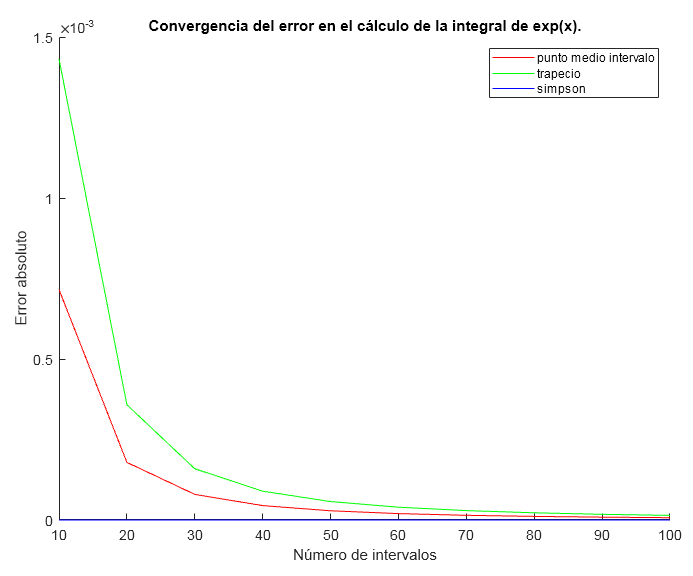
\includegraphics[width=\linewidth]{Integracion/error_int.png}
  \caption{Disminución del error al aumentar el número de intervalos (no se incluyen métodos con un error mayor).}
  \label{errorIntFig}
\end{figure}

\subsection{Apartado B}
Aplicamos los métodos al cálculo de \(\int_{0}^{2\pi} cos(x^2 - 1) \,dx\) y los comparamos con el valor exacto y la aproximación computados con:
\begin{lstlisting}
fB=@(x) cos((x.^2) - 1);
X = 0:pi/1000:2*pi;
Y = arrayfun(fB,X);
aproxiB = trapz(X,Y);
exactoB = integral(fB, 0, 2*pi);
\end{lstlisting}

Usando esta vez 2000 intervalos obtenemos unas conclusiones similares al apartado A (ver \autoref{tbl:errorIntB}).
\begin{table}
\begin{center}
\begin{tabular}{ |c|c| } 
 \hline 
 Metodo & abs(exacto-resultado) \\ 
 \hline \hline
 Rectángulo izquierda &  $2.7603\times10^{-04}$ \\ 
 \hline
 Rectángulo derecha &  $2.615\times10^{-04}$ \\ 
 \hline
 Rectángulo punto medio &  $3.632\times10^{-06}$ \\ 
 \hline
 Trapecio &  $7.2638\times10^{-06}$ \\ 
 \hline
 Simpson &  $4.5356\times10^{-11}$ \\ 
 \hline
\end{tabular}
\end{center}
\caption{Error absoluto cometido para el apartado B con 2000 intervalos.}
\label{tbl:errorIntB}
\end{table}

No se incluye la gráfica del error en el caso del apartado B por ser muy similar a la ya mostrada en el apartado A con el mismo incremento en el número de intervalos.
\section{Hoja 2: Resolución numérica de sistemas lineales}

Para la resolución de los sistemas lineales dados para los apartados 1 y 2 implementamos los métodos de Jacobi y de Gauss-Seidel como funciones. Ambas reciben como parámetros la matriz A con los coeficientes y la matriz columna B con los valores resultado del sistema de ecuaciones Ax = B, una solución inicial \textbf{``sol''} para la iteración y el valor de tolerancia. Y ambas devuelven un vector solución y el número de iteraciones efecturadas, que nos servirá para medir la eficiencia del método.

\begin{lstlisting}[language=Matlab, caption={Método de Jacobi.},captionpos=b,texcl=true]
function [res,count] = Jacobi(A, B, sol, tolerancia)
    next=zeros(1,length(sol));
    for i = 1:length(A)
        suma = 0;
        for j = 1:length(sol)
            if(i ~= j)
                suma = suma + A(i,j)*sol(j);
            end
        end
        next(i) = (B(i)-suma)/A(i,i);
    end
    count = 1;
    other = 0;
    for i = 1:length(sol)
        if(abs(sol(i)-next(i)) > tolerancia)
            [next, other] = Jacobi(A,B, next,tolerancia);
            break
        end
    end
    count = count + other;
    res = next;
end
\end{lstlisting}

\begin{lstlisting}[language=Matlab, caption={Método de Gauss-Seidel.},captionpos=b,texcl=true]
function [res, count] = GaussSeidel(A, B, sol, tolerancia)
    next = sol;
    for i = 1:length(A)
        suma = 0;
        for j = 1:length(next)
            if(i ~= j)
                if(i > j)
                    suma = suma + A(i,j)*next(j);
                else
                   suma = suma + A(i,j)*sol(j);
                end
            end
        end
        next(i) = (B(i)-suma)/A(i,i);
    end
    count = 1;
    other = 0;
    for i = 1:length(next)
        if(abs(sol(i)-next(i)) > tolerancia)
            [next, other] = GaussSeidel(A,B,next, tolerancia);
            break
        end
    end
    count = count + other;
    res = next;
end
\end{lstlisting}

\subsection{Apartado 1}

Para el sistema de ecuaciones dado (que no incluiremos aquí por brevedad) la solución obtenida con ambos métodos es \[x_1=3 , x_2=-2.5 , x_3=7\] pero con Gauss-Seidel obtenemos la solución en 3 iteraciones mientras que con el método de Jacobi usamos 4 con la misma toleracia de 0.01.

\subsection{Apartado 2}

Para el segundo sistema de cuatro ecuaciones con cuatro incógnitas podemos observar que Gauss-Seidel se aproxima a la solución de manera mucho más rápida y obtiene mejores resultados al reutilizar los valores de las variables ya computadas durante la iteración.

La solución dada en el enunciado es: \[x_1=2.7273 , x_2 = 0.4040 , x_3 = 0.6364 , x_4 = 0.1919\] es la usada para computar el error.
\begin{table}
\begin{center}
\begin{tabular}{ |c|c|c|c| } 
 \hline 
 Metodo & Tolerancia & Iteraciones (k) & max(Error\textsuperscript{k} \%) \\ 
 \hline \hline
 Jacobi &  0.1 & 5 & > 100 \\
 \hline
 Jacobi &  0.01 & 12 & 17.46\\
 \hline
 Jacobi &  0.001 & 21 & 1.19\\
 \hline
 Jacobi &  0.0001 & 29 & 0.1155\\
 \hline
 Gauss-Seidel & 0.1 & 4 & 31.9828\\
 \hline
 Gauss-Seidel & 0.01 & 8 & 3.0241\\
 \hline
 Gauss-Seidel & 0.001 & 12 & 0.3491\\
 \hline
 Gauss-Seidel & 0.0001 & 16 &  0.0335\\
 \hline
\end{tabular}
\end{center}
\caption{Interaciones y error \% según la tolerancia para Jacobi y Gauss-Seidel.}
\end{table}
\section{Hoja 3: Raíces numéricas de funciones no lineales}

A continuación se va a explicar la resolución de la práctica 3.
Para esta práctica se han programado en \textit{Matlab} dos métodos para encontrar las raíces numéricas de funciones no lineales.
El método de bisección y el método de Newton-Raphson.

\subsection{Método de bisección}
Partiendo de una función \(f(x)\) que este definida y sea continua en el intervalo \([x_1, x_2]\) tal que el signo de \(f(x_1)\) es distinto al de \(f(x_2)\) ó \(f(x_1)f(x_2) < 0\). Según el teorema de Bolzano-Weierstrass, dentro del intervalo \((x_1, x_2)\) tiene que existir al menos un valor de \(x\) tal que \(f(x) = 0\).

El método de bisección es un método iterativo en el que en cada iteración se realizan los siguientes pasos:

\begin{enumerate}
    \item Se calcula el punto medio \(m\) del intervalo como \(m = (x_1 + x_2)/2\).
    \item Si \(f(m) = 0\) entonces \(m\) es una raíz y se termina el algoritmo. Si no, se calcula el signo de \(f(m)\)
    \item En el intervalo actual \([x_1, x_2]\) se reemplaza o \(x_1\) o \(x_2\) con \(m\) tal que se siga cumpliendo que \(f(x_1)f(x_2) < 0\) para el nuevo intervalo.
    \item Se continua hasta el número de iteraciones determinado o hasta que el error sea menor que la cota predefinida.
\end{enumerate}

Usando superíndices para representar la iteración, el máximo error que se puede cometer dentro de un intervalo \([x_1^0, x_2^0]\) es \(e^1 = x_2^1 - x_1^1\) ó \(e^1 = (x_2^0 - x_2^0)/2\). Después de la \(n\) iteración, el error se puede calcular como

\[e^n = (x_2^0 - x_1^0)/2^n\]

El número de iteraciones \(n\) para que el error sea inferior a un valor \(\epsilon\) viene dado por
\[n >= \ln((x_2^0 - x_1^0) / \epsilon) / \ln(2)\]

\begin{lstlisting}[language=Matlab, caption={Algorítmo de bisección.},captionpos=b,texcl=true]
function res = Bisection(f, interval, error)
	iter = 0;
	totalIters = log((interval(2)-interval(1))/error)/log(2);

	while(iter < totalIters)
		xm = abs((interval(2)-interval(1))/2.0) + interval(1);

		if(f(xm) == 0.000)
			res = xm;
			break;
		elseif(sign(f(xm)) == sign(f(interval(2))))
			interval(2) = xm;
		elseif(sign(f(xm)) == sign(f(interval(1))))
			interval(1) = xm;
		end
		res = xm;
		iter = iter + 1;
	end
end
\end{lstlisting}

\subsection{Método de Newton-Raphson}
Dada una función de valores reales que sea continua y diferenciable, el método se basa en coger un punto inicial \((x_0^0, f(x_0^0))\) y seguir la derivada de \(f(x)\) en dicho punto en cada iteración de tal manera que el resultado de la iteración número \(n\) viene dado por la ecuación.

\[x_0^n = x_0^{n-1} - \frac{ f(x_0^{n-1}) } { f'(x_0^{n-1}) } \]

Este método puede no funcionar si alrededor del punto \(x\) o de la raíz existen máximos, mínimos o puntos de inflexión (\(f'(x) = 0\)).

El error estimado \(\epsilon\) en una iteración \(n\) se ha calculado como \(\epsilon_n = | x_n - x_{n-1} | \).

\begin{lstlisting}[language=Matlab, caption={Algorítmo de Newton-Raphson},captionpos=b,texcl=true]
function res = NewtonRaphson(f, df, startX, error)
	newX = startX;
	keepGoing = true;
	while(keepGoing)
		newX = startX - (f(startX) / df(startX));
		if ( abs(newX - startX) < error)
			keepGoing = false;
		end
		startX = newX;
	end
	res = newX;
end
\end{lstlisting}

\subsection{Resultados}

\subsubsection{Ejercicio A}

\begin{figure}[H]
    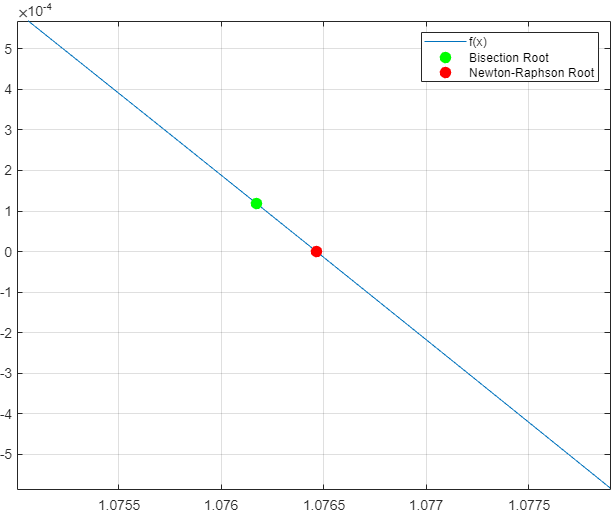
\includegraphics[width=8cm]{NumRoots/NumRoots_A}
    \centering
\end{figure}

\subsubsection{Ejercicio B}

\begin{figure}[H]
    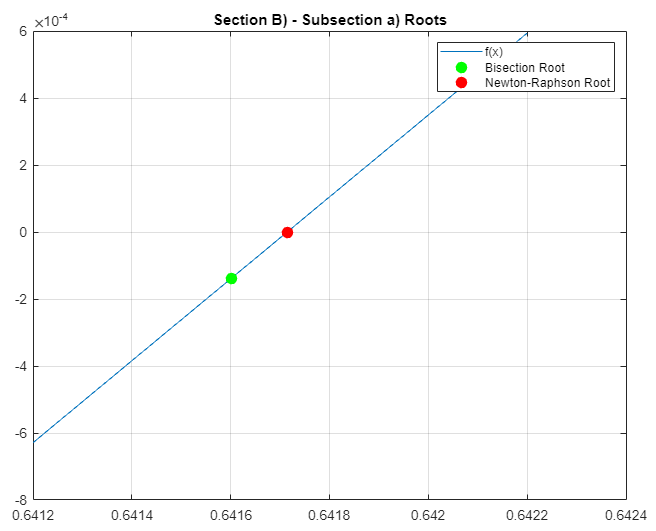
\includegraphics[width=10cm]{NumRoots/NumRoots_Ba}
    \centering
\end{figure}

\begin{figure}[H]
    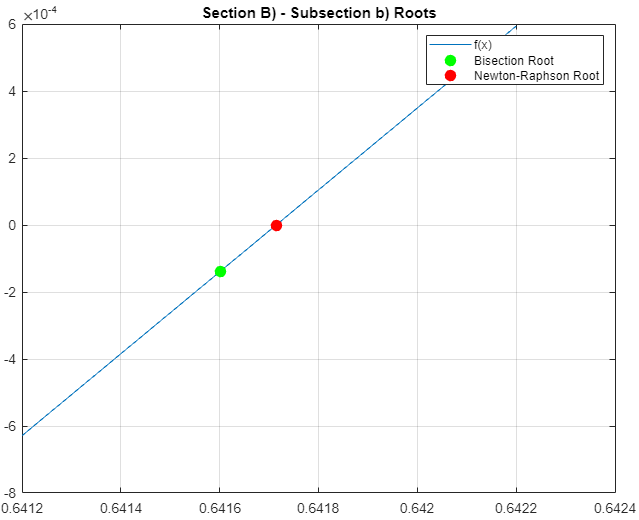
\includegraphics[width=10cm]{NumRoots/NumRoots_Bb}
    \centering
\end{figure}

\subsubsection{Ejercicio C}

\begin{figure}[H]
    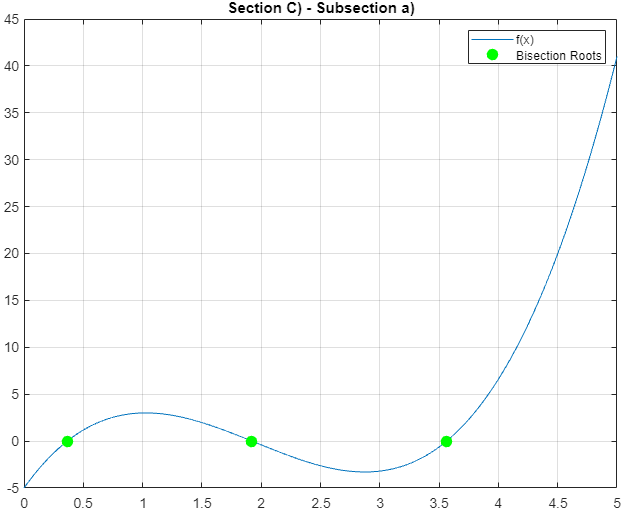
\includegraphics[width=10cm]{NumRoots/NumRoots_Ca}
    \centering
\end{figure}

\begin{figure}[H]
    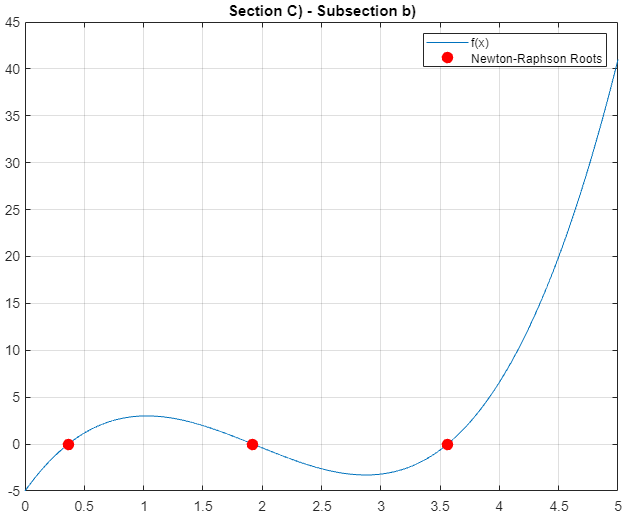
\includegraphics[width=10cm]{NumRoots/NumRoots_Cb}
    \centering
\end{figure}

\subsubsection{Ejercicio D}

\begin{figure}[H]
    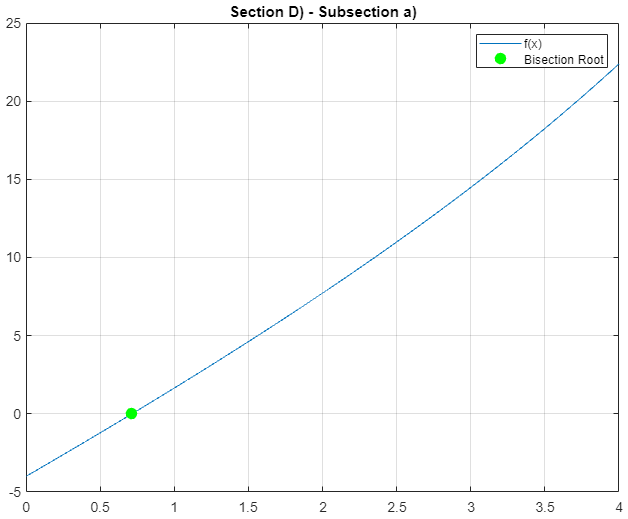
\includegraphics[width=10cm]{NumRoots/NumRoots_Da}
    \centering
\end{figure}

\begin{figure}[H]
    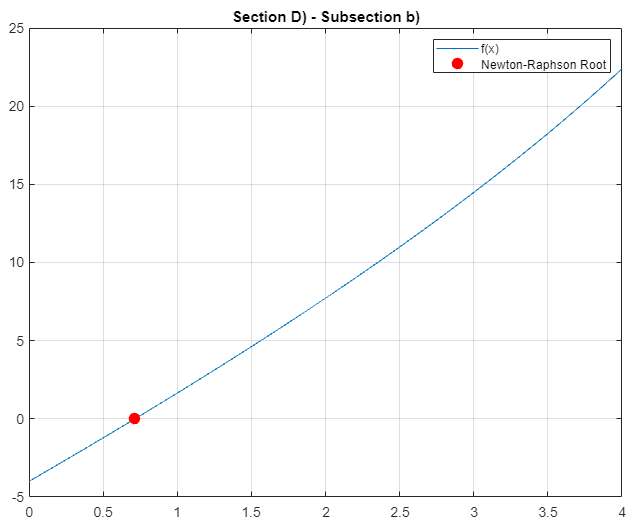
\includegraphics[width=10cm]{NumRoots/NumRoots_Db}
    \centering
\end{figure}
\section{Hoja 4: Métodos de integración numérica: Euler explícito}
\label{sec:metodos-de-1-paso:-euler}

A continuación se va a explicar la resolución de la práctica 4.

\subsection{Método de Euler explícito}\label{subsec:metodo-de-euler-explicito}

Dada una función \(f'(x)\) definida en el intervalo \([x_0, x_f]\) cuya
integral sea inviable calcular de forma analítica y un valor inicial en la integral
\(f(x_0)\ = y_0\), se divide el intervalo a integrar en \(n\) sub-intervalos
de ancho \(h\); es decir: \[h = \frac{x_f - x_0}{n}\]
de manera que se consigue un conjunto discreto de puntos de tamaño \(n+1\)
donde se cumple que: \[x_i = x_0 + ih \quad 0 \leq i \leq n\]

Se define la aproximación de la integral discreta \(f(x)\) definida en
los puntos \(x_i\) tal que: \[f(x_{i+1}) = f(x_i) + h * f'(x_i)\]

\subsection{Método de Euler explícito en ecuaciones diferenciales}
\label{subsec:metodo-de-euler-explicito-en-ecuaciones-diferenciales}

Dada la ecuación definida como \[\frac{dy}{dt} = f(y, t)\] y el punto \(y(t_0) = y_0\)
se puede emplear el método de Euler explícito para obtener resultados aproximados
discretos en el intervalo \([y_0, y_f]\).
Para ello, se debe primero elegir un número de sub-intervalos \(n\) y calcular
el ancho de cada intervalo \(h\).
Una vez calculados los sub-intervalos, se deben calcular los valores aproximados
de cada intervalo iterando la siguiente fórmula:
\[y_{i+1} = y_i + h * f(y_i, t_i)\]
siendo \(t_i = t_0 + h * i\).

Este método puede ser implementado en \textit{MatLab} de la siguiente manera:

\begin{lstlisting}[language=Matlab, caption={Método de Euler explícito.},captionpos=b,
    texcl=true,label={lst:lstlisting}]
function f = explicit_euler (fun, h, y)
    f = y + h * fun;
end
\end{lstlisting}

siendo \(fun\) la ecuación diferencial definida de la manera anteriormente mencionada,
\(h\) el ancho de cada sub-intervalo e \(y\) la variable simbólica que se debe integrar.

\subsection{Problema 1}\label{subsec:problema-1}

En este primer problema se debe resolver el siguiente problema diferencial de Cauchy
por el método de Euler explícito con \(h = 0.2\):

\[
    \begin{cases}
        y' = y - t^2 + 1 \quad 0 < t < 1 \\
        y(0) = 0.5
    \end{cases}
\]

Sabiendo que la solución exacta es \[y(t) = (t + 1)^2 - 0.5e^t\]
se debe elaborar una tabla de datos que incluya los puntos de soporte, los valores
exactos de la solución, los valores aproximados de la solución y el error cometido relativo.
También se debe representar gráficamente la aproximación y la solución exacta.
Por último, se debe estudiar la convergencia del método variando el valor de \(h\) hacia
valores más pequeños.

El resultado para \(h = 0.2\) es el siguiente:

\begin{table}[H]
    \begin{center}
        \begin{tabular}{ |c|c|c|c|c| }
            \hline
            Índice & Punto & Valor aproximado & Valor real & Error relativo \\
            \hline
            \hline
            1      & 0     & 0.5              & 0.5        & 0              \\
            \hline
            2      & 0.2   & 0.792            & 0.8293     & 0.044976       \\
            \hline
            3      & 0.4   & 1.1184           & 1.2141     & 0.078814       \\
            \hline
            4      & 0.6   & 1.4701           & 1.6489     & 0.10847        \\
            \hline
            5      & 0.8   & 1.8361           & 2.1272     & 0.13686        \\
            \hline
        \end{tabular}
    \end{center}
    \caption{Tabla del ejercicio 1 con \(h = 0.2\)}\label{tab:euler-1-0-2}
\end{table}

\begin{figure}[H]
    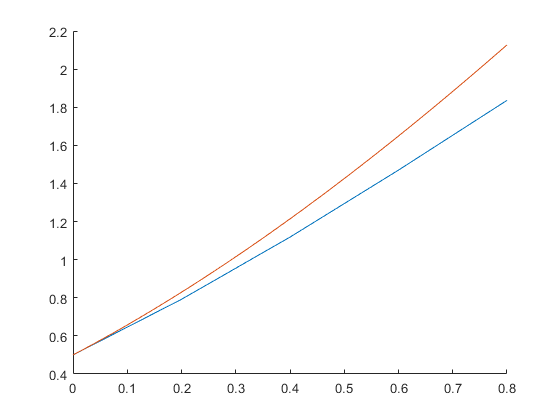
\includegraphics[width=8cm]{Euler/Euler102}
    \centering
    \caption{Resultado del ejercicio 1 con \(h = 0.2\)}\label{fig:euler-1-0-2}
\end{figure}

Si disminuimos el valor de \(h\), se observa como la aproximación converge
a la función original.

\begin{table}[H]
    \begin{center}
        \begin{tabular}{ |c|c|c|c|c| }
            \hline
            Índice & Punto & Valor aproximado & Valor real & Error relativo \\
            \hline
            \hline
            1      & 0     & 0.5              & 0.5        & 0              \\
            \hline
            2      & 0.1   & 0.649            & 0.65741    & 0.012799       \\
            \hline
            3      & 0.2   & 0.8099           & 0.8293     & 0.023392       \\
            \hline
            4      & 0.3   & 0.98189          & 1.0151     & 0.032688       \\
            \hline
            5      & 0.4   & 1.1641           & 1.2141     & 0.04119        \\
            \hline
            6      & 0.5   & 1.3555           & 1.4256     & 0.049208       \\
            \hline
            7      & 0.6   & 1.555            & 1.6489     & 0.056949       \\
            \hline
            8      & 0.7   & 1.7615           & 1.8831     & 0.064565       \\
            \hline
            9      & 0.8   & 1.9737           & 2.1272     & 0.072177       \\
            \hline
            10     & 0.9   & 2.1901           & 2.3802     & 0.079882       \\
            \hline
        \end{tabular}
    \end{center}
    \caption{Tabla del ejercicio 1 con \(h = 0.1\)}\label{tab:euler-1-0-1}
\end{table}

\begin{figure}[H]
    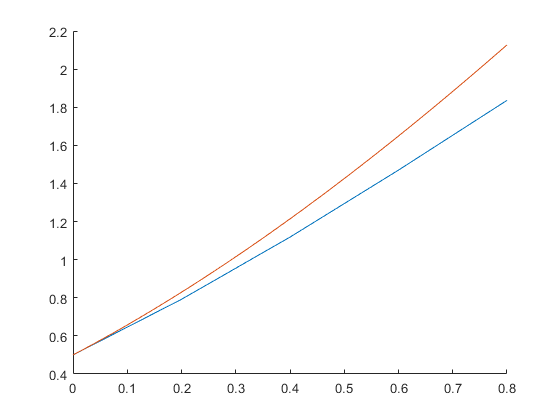
\includegraphics[width=8cm]{Euler/Euler102}
    \centering
    \caption{Resultado del ejercicio 1 con \(h = 0.1\)}\label{fig:euler-1-0-1}
\end{figure}

\begin{table}[H]
    \begin{center}
        \begin{tabular}{ |c|c|c|c|c| }
            \hline
            Índice & Punto  & Valor aproximado & Valor real & Error relativo \\
            \hline
            \hline
            1      & 0      & 0.5              & 0.5        & 0              \\
            \hline
            2      & 0.01   & 0.515            & 0.51507    & 0.00014739     \\
            \hline
            3      & 0.02   & 0.53014          & 0.5303     & 0.00029104     \\
            \hline
            4      & 0.03   & 0.54544          & 0.54567    & 0.0004312      \\
            \hline
            5      & 0.04   & 0.56088          & 0.56119    & 0.00056807     \\
            \hline
            6      & 0.05   & 0.57646          & 0.57686    & 0.00070186     \\
            \hline
            \ldots & \ldots & \ldots           & \ldots     & \ldots         \\
            \hline
            96     & 0.95   & 2.4874           & 2.5096     & 0.0088767      \\
            \hline
            97     & 0.96   & 2.513            & 2.5358     & 0.0089624      \\
            \hline
            98     & 0.97   & 2.5387           & 2.5619     & 0.0090483      \\
            \hline
            99     & 0.98   & 2.5645           & 2.5882     & 0.0091345      \\
            \hline
            100    & 0.99   & 2.5904           & 2.6145     & 0.0092211      \\
            \hline
        \end{tabular}
    \end{center}
    \caption{Tabla del ejercicio 1 con \(h = 0.01\)}\label{tab:euler-1-0-0-1}
\end{table}

\begin{figure}[H]
    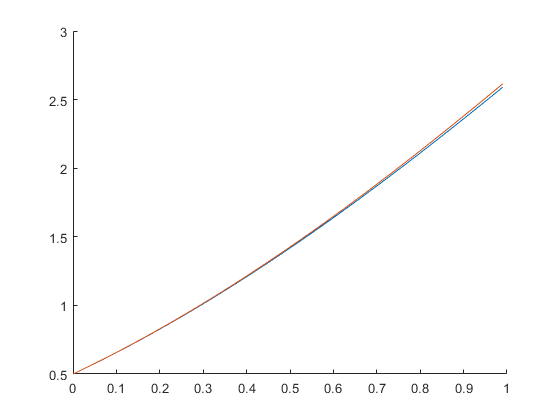
\includegraphics[width=8cm]{Euler/Euler1001}
    \centering
    \caption{Resultado del ejercicio 1 con \(h = 0.01\)}\label{fig:euler-1-0-0-1}
\end{figure}

\subsection{Problema 2}\label{subsec:problema-2}

En el segundo problema se debe resolver el siguiente problema diferencial de Cauchy de
orden 2 por el método de Euler explícito con \(h = 0.05\) y \(T = 0.1\):

\[
    \begin{cases}
        Mu'' = B|u'|u' + ku \quad 0 < t < T \\
        u(0) = u_0
        u'(0) = u_{p0}
    \end{cases}
\]

Se deben usar las constantes \(M = 10 kg\), \(B = 50 Ns^2/m^2\), \(k = 200 N/m\),
\(u_0 = 0\) y \(u_{p0} = 1 m/s\).

Al ser \(h = 0.05\) y \(T = 0.1\), el programa solo ha de integrar una única vez
en el punto \(x = 0.05\).
La gráfica resultante es la siguiente:

\begin{figure}[H]
    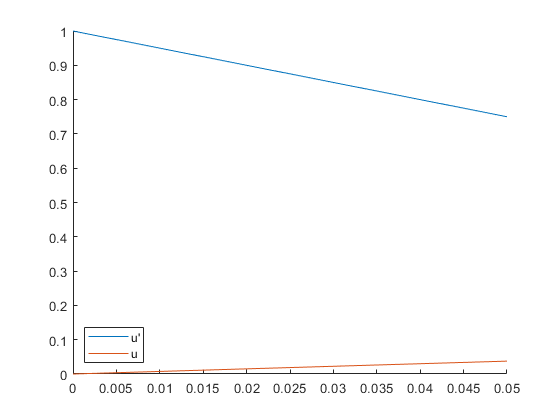
\includegraphics[width=8cm]{Euler/Euler2}
    \centering
    \caption{Resultado del ejercicio 2}\label{fig:euler-2}
\end{figure}

Las variables que más influyen en la ecuación son \(M\) y \(B\).
Si se disminuye el valor de \(M\) y se aumenta el valor de \(B\)
el valor de \(u'\) disminuye considerablemente.

\begin{figure}[H]
    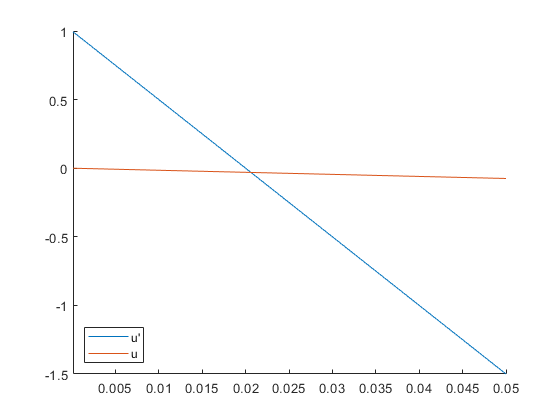
\includegraphics[width=8cm]{Euler/Euler22}
    \centering
    \caption{Resultado del ejercicio 2 con \(M\) disminuido y \(B\) aumentado}
    \label{fig:euler-22}
\end{figure}



\end{document}

